\chapter{Approximations}
\graphicspath{{../gfx/chapter02/}{../plots/chapter02/}}

% TODO: in chapter 1: change V_2 -> V_0
% TODO: chapter one, decomposed Hamiltonian: - H^c_k -> + H^c_k
% TODO: consistent \emph{fixed charge} terminology

\section{Fixed charge model}

Exact diagonalization scales exponentially with system size. For the full
\emph{grand canonical} QCA Hamiltonian, Eq.~\ref{eq:H_QCA}, only QCA devices of
up to two cells are computationally feasible. Therefore, to access larger
systems we need to introduce approximations. Approximating means to simplify.
However, by carefully establishing successive approximations and their limits,
we also reduce the problem to its essential ingredients and thus, hopefully, we
gain a better understanding of the system. As a first step, we reduce the
Hilbert space to a \emph{fixed} number of particles per cell. We disallow any
charge fluctuations, both for the system as a whole and for each individual
cell. With that, we omit the chemical potential term in the Hamiltonian, $\mu =
0$, and prohibit inter-cell hopping. This is a major simplification. However, it
is in line with the QCA idea: The approach requires a fixed number of charges
per cell, typically two electrons, and cells are thought to interact only via
Coulomb forces. In a sense we are shifting the starting point of our
investigation. If the \emph{fixed} charge approximation is not valid for a given
system, then there is no hope of implementing QCA on it. On the other hand, for
experimental systems like the atomic silicon quantum dots and for a given cell
layout, it should always be possible, at least in principle, to tune the system
parameters, especially the chemical potential, to get the system into the right
particle number sector. The system has to be set up in a way that the
two-electrons-per-cell sector is lowest in energy and other particle number
sectors are sufficiently gapped out, that is, at an energy, compared to the
ground state energy, much larger than temperature. Of course, in practice there
are very clear limits as to how much the system parameters can be tuned and any
QCA cell layout considered within the \emph{fixed} charge approximation cannot
necessarily be readily implemented on a given real-world material system.

For the \emph{fixed} charge system, the state space scales as $N_s =
\binom{8}{2}^{N_c} = 28^{N_c}$ ($N_c$ is the number of cells). Using symmetries,
the largest block of the Hamiltonian matrix is the spin zero sector, of size
$N_s^{\prime} = 16^{N_c}$. On conventional computer hardware, systems of up to
four cells are possible, with memory requirements of 32GB. In practice,
however, calculations for four-cell systems take too long and thus three
cells is the practical limit for the \emph{fixed}-number-of-particles-per-cell
model.


\section{Bond model}

%
\begin{figure}
  % TODO: include numbering of states, e.g. \ket{1}, and so on
  \center
  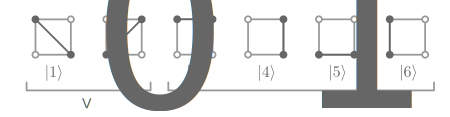
\includegraphics{bond}
  \caption{\ldots}
  \label{fig:bond}
\end{figure}
%
At its heart, QCA is a semi-classical idea. It relies solely on charge-charge
interactions and ignores the particle spins. Therefore, as a next step in our
quest to access larger system sizes, we neglect the spin degree of freedom in
our model. The 28 states per cell of the \emph{fixed} charge model can be
reorganized into four doubly occupied dots and six bonds. The six bonds are
illustrated in Fig.~\ref{fig:bond}. Each bond corresponds to one spin singlet
and three spin triplet states. The \emph{bond} approximation only keeps one
state for each bond and discards the doubly occupied states as well. With the
\emph{bond} model we thus assume that singlet and triplet states are
qualitatively equivalent and energetically degenerate, and that doubly occupied
dots are sufficiently gapped out, that is, $U \gg T$. As QCA ignores the spin,
singlets and triplets should be qualitatively equivalent, but they are not quite
degenerate. We expect that virtual double-occupancy lowers the energies of the
singlet states and therefore introduces a small singlet-triplet splitting.
Still, degeneracy is presumably not a bad assumption to start with and we will
look at the singlet-triplet splitting in detail in due course. For the
\emph{bond} model the QCA Hamiltonian reduces to
%
\begin{equation}
  \label{eq:H_bond}
  H = - \sum_{\left<ij\right>} t c_i^{\dagger} c_j
      + \sum_{i<j} V_{ij} \left( n_i - q \right) \left( n_j - q \right) \, .
\end{equation}
%
With six bond states per cell, the Hilbert space of the \emph{bond} model is
$N_s = 6^{N_c}$ ($N_c$ the number of cells). Five and six cells are doable, with
memory requirements of 460MB and 16GB, respectively, but for practical
calculations five cells really is the limit. For the \emph{bond} model there are
no symmetries that can be exploited.


\section{Ising model}

\newcommand{\ket}[1]{\left|#1\right>}
\newcommand{\bra}[1]{\left<#1\right|}

%
\begin{figure}
  \center
  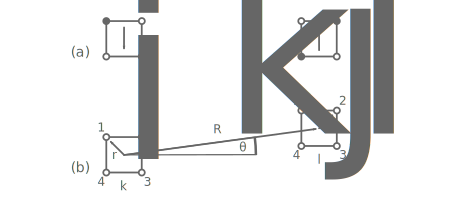
\includegraphics{ising}
  \caption{a) QCA cells $k$ and $l$. b) The two-states-per-cell approximation
  identifies each cell with a spin $\uparrow$ or $\downarrow$.}
  \label{fig:cells2}
\end{figure}
%
A linear array of QCA cells where each cell has a state of logic 0 or 1 is
reminiscent of a 1D spin $\frac{1}{2}$ chain. Indeed, if we reduce the basis to
only two states per cell, down from six states in the \emph{bond} picture, we
can map the QCA system to a transverse-field Ising model with long-ranging
interactions. This is an attractive proposition: The smaller Hilbert space
allows for larger system sizes with our exact diagonalization method; more
importantly, the transverse-field Ising model is amenable to sign-problem-free
Stochastic series expansion (SSE) quantum Monte Carlo schemes
\cite{Sandvik2003}. These methods do not scale exponentially\footnote{SSE
quantum Monte Carlo methods roughly scale as $N \ln N$ where $N$ is the system
size.} and consequently allow access to much larger systems. Last, but not
least, such a mapping connects the QCA approach to the established and well
studied Ising model. The prospect hinges on the assumption that the
two-states-per-cell basis actually is a good approximation for QCA systems. And
while bistable two-state cells are certainly the picture we have in mind when we
talk about QCA, it is not \emph{a priori} clear whether this is a correct
physical picture. 

We use the \emph{bond} Hamiltonian \eqref{eq:H_bond} as the starting point. We
had already discussed in the last chapter that such a Hamiltonian can be
decomposed into single-cell terms and cell-cell interaction terms,
\begin{equation}
  H = \sum_k H^c_k + \sum_{k<l} H^{cc}_{kl} \, .
\end{equation}
In comparison, the transverse field Ising model is described by
%
\begin{equation}
  \tilde{H} = - \sum_k \gamma S^x_k + \sum_{k<l} J_{kl} S^z_k S^z_l \, .
\end{equation}
%
Thus, we would like to map the single cell term $H^c_k$ to the transverse field
term $-\gamma S^x_k$ and the Coulombic cell-cell interaction $H^{cc}_{kl}$ to 
the Ising term $J_{kl} S^z_k S^z_l$. Each cell $k$ is identified with a pseudo
spin $S^z_k$, specifically the logic 0 with a spin down state and the logic 1
with a spin up state, as illustrated in Fig.~\ref{fig:cells2}(b). We will first
look at how the QCA cell can be represented by only two states and derive an
approximate expression for the transverse field $\gamma$. Then we will use a
multipole expansion to derive $J_{kl}$ from the cell-cell Coulomb interaction.
% TODO: maybe point out again that J_{kl} is long-ranged

To arrive at a single-cell-basis with only two states we can, in principle,
follow a similar prescription as for the fixed charge and bond approximations:
We neglect high energy states which are assumed to be gapped out. In this case
these are the four edge states with Coulomb energy $V_1$, $\ket{\psi_Q} =
\left\{ \ket{3}, \ket{4}, \ket{5}, \ket{6} \right\}$ in Fig.~\ref{fig:bond},
where we have introduced $\ket{\psi_Q}$ to denote the high-energy subspace of
the single-cell Hilbert space. We only keep the low-energy, diagonal states
$\ket{\psi_P} = \left\{ \ket{1}, \ket{2} \right\}$ with Coulomb energy $V_0$. Of
course, these two are exactly our logic 0 and logic 1 state, or $\ket{1} \doteq
\ket{\downarrow}$ and $\ket{2} \doteq \ket{uparrow}$, respectively.  Here,
$\ket{\psi_P}$ denotes the low-energy subspace. For the high-energy states to be
sufficiently gapped out we require $\Delta V = V_1 - V_0 \gg T$. In contrast to
the fixed charge and bond models, merely truncating the Hilbert space is not
sufficient for the Ising model. For our previous two approximations the
Hamiltonian had remained essentially unchanged, apart from dropping no longer
relevant terms, such as the chemical potential term or the Hubbard $U$ term. The
retained states were exactly the same states as in the full, untruncated model.
But with only two states per cell the existing Hamiltonian \eqref{eq:H_bond}
does not ``work'': There is no process that takes the system from state
$\ket{1}$ to $\ket{2}$. Therefore, for the Ising approximation we need to derive
an effective, low-energy Hamiltonian from the bond model. In the bond picture,
for the system to transition from state $\ket{1}$ to $\ket{2}$ it can take
different paths, for example $\ket{1} \rightarrow \ket{3} \rightarrow{2}$,
consisting of two hopping processes with an interim high-energy edge state. We
will treat those processes perturbatively, as \emph{virtual} excitations, and
derive an effective hopping term between the two states $\ket{1}$ and $\ket{2}$.
This effective hopping term is precisely the transverse field $\gamma$ which
flips the spin in the Ising picture, $-\gamma S^x_k = -\gamma \frac{1}{2} \left(
S^+_k + S^-_k \right)$.

A single QCA cell is described by the time-independent Schr\"odinger equation
$H^c_k \ket{\psi} = E_k \ket{\psi}$, with $\ket{\psi} = \left[ \ket{\psi_P}
\ket{\psi_Q} \right]$. Our aim it to truncate the basis to $\ket{\psi_P}$ and
derive and an effective Hamiltonian $\tilde{H}^c_k$ with the subspace
Schr\"odinger equation $\tilde{H}^c_k \ket{\psi_p} = E_k \ket{\psi_p}$. The
high-energy states $\ket{\psi_Q}$ have to be incorporated as virtual
excitations.  Using the basis depicted in Fig.~\ref{fig:bond} the single-cell
bond Hamiltonian is very simple and can be written down explicitly. As the
single-cell Hamiltonian is the same for all cells, we can drop the index $k$.
%
\begin{equation}
\begin{split}
  \label{eq:H_marix}
  H^c
  &=
  %
  \left(
  \begin{array}{cc|cccc}
    V_0 & 0   & -t  & -t  & -t  & -t  \\
    0   & V_0 & -t  & -t  & -t  & -t  \\
    \hline
    -t  & -t  & V_1 & 0   & 0   & 0   \\
    -t  & -t  & 0   & V_1 & 0   & 0   \\
    -t  & -t  & 0   & 0   & V_1 & 0   \\
    -t  & -t  & 0   & 0   & 0   & V_1 \\
  \end{array}
  \right) \\[1em]
  %
  &=
  \left(
  \begin{array}{cc}
    H_{PP} & H_{PQ} \\
    H_{QP} & H_{QQ} \\
  \end{array}
  \right)
\end{split}
\end{equation}
%
Here, we have partitioned the Hamiltonian into four blocks, $H_{PP}$, $H_{QQ}$,
$H_{PQ}$, and $H_{QP}$, corresponding to the low-energy subspace $\ket{\psi_P}$,
the high-energy subspace $\ket{\psi_Q}$, and transitioning between the subspaces.
With a this partitioned Hamiltonian the time-independent Schr\"odinger equation
is
%
\begin{equation}
  \label{eq:SE}
  %
  \begin{pmatrix}
    H_{PP} & H_{PQ} \\
    H_{QP} & H_{QQ} \\
  \end{pmatrix}
  \begin{pmatrix}
    \psi_P \\
    \psi_Q \\
  \end{pmatrix}
  =
  E
  \begin{pmatrix}
    \psi_P \\
    \psi_Q \\
  \end{pmatrix}
  %
\end{equation}
%
Writing out the matrix equation as two equations explicitly and eliminating
$\ket{\psi_Q}$ yields 
%
\begin{equation}
  H_{PP} \ket{\psi_P} + H_{PQ} \frac{1}{E - H_{QQ}} H_{QP} \ket{\psi_P}
  =
  E \ket{\psi_P}
\end{equation}
%
and therefore
%
\begin{equation}
  \label{eq:H_effective}
  \tilde{H}^c = H_{PP} + H_{PQ} \frac{1}{E - H_{QQ}} H_{QP} \, .
\end{equation}
%
Assuming that the system is predominantly in the subspace spanned by
$\ket{\psi_P}$ and additionally that the hopping is very small, $t \ll V_0$, we
can approximate $E \approx V_0$. We write out the matrix multiplications and use
$H_{PP} = \left( V_0 \right)_{ii} \delta_{ij}$, $H_{PQ} = \left( -t
\right)_{ij}$, and so on. The effective Hamiltonian becomes
%
\begin{equation}
\begin{split}
  \tilde{H}^c_{ij}
  %
  &=
  \left( V_0 \right)_{ii} \delta_{ij}
  + \left( - t \right)_{ik}
    \left( V_0 - V_1 \right)^{-1}_{kk}
    \left( - t \right)_{kj} \\
  %
  &=
  \left( V_0 \right)_{ii} \delta_{ij}
  - \left( \frac{4 t^2}{\Delta V} \right)_{ij} \, .
\end{split}
\end{equation}
%
As the system remains unchanged upon adding a constant term to the Hamiltonian,
we can subtract the constant diagonal term $\tilde{H}_{ii} = V_0 - \frac{4
t^2}{\Delta V}$, and arrive at
%
\begin{equation}
  \tilde{H}^c
  =
  \begin{pmatrix}
    0 & - \frac{4 t^2}{\Delta V} \\
    - \frac{4 t^2}{\Delta V} & 0 \\
  \end{pmatrix} \, .
\end{equation}
%
The off-diagonal matrix elements are the effective hopping, transitioning the
system between its two states $\ket{1} \leftrightarrow \ket{2}$. If we now
compare this matrix with the transverse field term of the Ising model, where we
use the basis $\ket{\downarrow} \doteq \ket{1}$ and $\ket{\uparrow} \doteq
\ket{2}$, 
%
\begin{equation}
\begin{split}
  \tilde{H}^c
  &=
  - \gamma S^x_k \\
  &=
  - \frac{1}{2} \gamma \left( S^+_k + S^-_k \right) \\[0.5em]
  &= 
  \begin{pmatrix}
    0 & - \frac{1}{2} \gamma \\
    - \frac{1}{2} \gamma & 0 \\
  \end{pmatrix} \, ,
\end{split}
\end{equation}
%
we identify the effective hopping as the transverse field $\gamma$
%
\begin{equation}
  \label{eq:gamma}
  \gamma = \frac{8 t^2}{\Delta V} \, .
\end{equation}
%
The effective hopping $\gamma$ is a virtual process, involving two hopping
processes in the original bond model, yielding the $t^2$ in the numerator of the
expression for $\gamma$, and an interim high-energy state gapped out by $\Delta
V$, hence the $\Delta V$ in the denominator. To arrive at the expression for the
effective hopping we used the assumptions $\Delta V \gg T$ and $t \ll \Delta V$.
As a reminder, $\Delta V = V_1 - V_0 = \frac{2 - \sqrt{2}}{2} \frac{1}{a}
\approx 0.3 V_1$. Notably, the energy gap is independent of the compensation
charge $q$. As the derivation used only a single cell, it is also implicitely
assumed that the perturbations from other cells in the system are small, at
least as far as the effective hopping is concerned. If the hopping depended on
nearby cells' state, then the effective Hamiltonian would be much more involved
and certainly could not be mapped to an Ising-like model.

We have successfully derived an effective hopping term and therefore also an
effective two-state model for the QCA Hamiltonian. With only two states per cell
the Hilbert space scales as $N_s = 2^{N_c}$ ($N_c$ the number of cells) and up
to 14 cells are computationally feasible, with memory requirements of 2GB. In
practice we restrict the calculations to a maximum of 12 or 13 cells. For our
calculations we can use the two-state approximation with the effective hopping
term, but still retain the original cell-cell interaction term $H^{cc}_{kl}$.
Summing up all cell-cell interactions exactly is no problem for the relatively
small system sizes accessible with exact diagonalization.  Thus, from a
computational point of view, nothing is gained by expressing the cell-cell
interaction as an Ising interaction. However, deriving $J_{kl}$ from
$H^{cc}_{kl}$ is very rewarding conceptually and enables us to properly map the
QCA approach to an Ising model. Additionally, an analytical expression for
$J_{kl}$ will already allow some key insights into the characteristics of QCA
devices. Therefore, we now undertake the derivation of an expression for
$J_{kl}$. The obvious starting point is the cell-cell interaction term
$H^{cc}_{kl}$, 
%
\begin{equation}
\begin{split}
  H^{cc}_{kl} 
  %
  &=
  %
  \sum_{\substack{i \in k\\j \in l}} V_{ij} \left( n_i - q \right) \left( n_j - q \right) \\
  %
  H^{cc}_{kl}
  %
  &= 
  %
  \sum_{\substack{i \in k\\j \in l}}
  \frac{ \left( n_i - q \right) \left( n_j - q \right) }
       { \left| \bm{R}_{kl} + \bm{r}_j - \bm{r}_i \right| } \\
  %
  &=
  \sum_{\substack{i \in k\\j \in l}}
  \frac{n_i n_j - q (n_i + n_j)}
       {\left| \bm{R}_{kl} + \bm{r}_{ij} \right|} \, ,
\end{split}
\end{equation}
%
where $i$ and $j$ sum over the four dots $1\ldots4$ of cell $k$ and $l$,
respectively, $\bm{R}_{kl}$ denotes the vector between the centres of the cells,
see Fig.~\ref{fig:cells2}(a). We have introduced $\bm{r}_{ij} = \bm{r}_j -
\bm{r}_i$ and dropped the constant $q^2$ term. There are only four possible
configurations for two interacting cells: $\uparrow\uparrow$,
$\downarrow\downarrow$, $\uparrow\downarrow$, and $\downarrow\uparrow$. Using
the shorthand notations $V_{ij} = \frac{1}{\left| \bm{R}_{kl} + r_{ij} \right|}
+ \frac{1}{\left| \bm{R}_{kl} - r_{ij} \right|}$ and $V_{00} = \frac{1}{\left|
\bm{R}_{kl} \right|}$, we calculate their energies explicitely.
\begin{align}
  %
  E^{\uparrow\uparrow}
  &=
  \left( 1 - 2 q \right) \left( 2 V_{00} + V_{24} \right)
  - q \left( 2 V_{12} + 2 V_{14} \right)
  \\
  %
  E^{\downarrow\downarrow}
  &=
  \left( 1 - 2 q \right) \left( 2 V_{00} + V_{13} \right)
  - q \left( 2 V_{12} + 2 V_{14} \right)
  \\
  %
  E^{\uparrow\downarrow}
  &=
  \left( 1 - 2 q \right) \left( V_{12} + V_{14} \right)
  - q \left( 4 V_{00} + V_{13} + V_{24} \right)
  \\
  %
  E^{\downarrow\uparrow}
  &=
  \left( 1 - 2 q \right) \left( V_{12} + V_{14} \right)
  - q \left( 4 V_{00} + V_{13} + V_{24} \right)
\end{align}
Note that the expression for two spin-down cells can be obtained from the
expression for two spin-up cells (and similarly ($E^{\uparrow\downarrow}$ from
$E^{\downarrow\uparrow}$) simply by rotating the system by $90^{\circ}$, or
equivalently by permuting the dot numbering, $1,2,3,4 \rightarrow 4,1,2,3$.
Symmetries can be exploited, for example $V_{43} = V_{12}$. Evidently,
$E^{\uparrow\downarrow} = E^{\downarrow\uparrow}$, which, given the highly
symmetric geometry of those cell arrangements, does not come as a surprise. But
crucially, we find $E^{\uparrow\uparrow} \ne E^{\downarrow\downarrow}$.
Therefore we have a system with three distinct energy levels which we cannot
hope to represent with the solely two-level Ising term $J_{kl} S^z_l S^z_l$.
Instead, let us try to map to a \emph{modified} Ising model with a three-level
cell-cell interaction term of the form
%
\begin{equation}
  \label{eq:Ising_term}
  %
  \tilde{H}^{cc}_{kl}
  = 
  J_{kl} S^z_k S^z_l + 
  J^{\prime}_{kl} \left( S^z_k + S^z_l \right) \, .
\end{equation}
%
For this Hamiltonian we have the energies
%
\begin{align}
  \tilde{E}^{\uparrow\uparrow} - \tilde{E}^{\uparrow\downarrow}
  &=
  2J_{kl} + 2J^{\prime}_{kl} \\
  %
  \tilde{E}^{\downarrow\downarrow} - \tilde{E}^{\uparrow\downarrow}
  &=
  2J_{kl} - 2J^{\prime}_{kl}
\end{align}
%
which yields
%
\begin{align}
  \label{eq:Js_from_Es}
  J_{kl}
  &=
  \frac{1}{4} 
  \left( 
    \tilde{E}^{\uparrow\uparrow} + \tilde{E}^{\downarrow\downarrow}
    - 2 \tilde{E}^{\uparrow\downarrow} 
  \right) \\
  %
  J^{\prime}_{kl}
  &=
  \frac{1}{4}
  \left( \tilde{E}^{\uparrow\uparrow} - \tilde{E}^{\downarrow\downarrow} \right) \, ,
\end{align}
%
and therefore, identifying $E^{\uparrow\uparrow} = \tilde{E}^{\uparrow\uparrow},
E^{\downarrow\downarrow} = \tilde{E}^{\downarrow\downarrow}$, and so on,
\begin{align}
  \label{eq:J}
  %
  J_{kl}
  &=
  \frac{1}{4} 
  \left(
    4 V_{00} + V_{13} + V_{24} - 2 V_{12} - 2 V_{14}
  \right) \\
  %
  \label{eq:Jprime}
  %
  J^{\prime}_{kl}
  &=
  \frac{1}{4}
  \left( 1 - 2 q \right)
  \left( V_{24} - V_{13} \right) \, .
\end{align}
These results, while abstract, are remarkable in two ways. First, the newly
introduced term $J^{\prime}_{kl}$ vanished for $q=\frac{1}{2}$. In this case
$E^{\uparrow\uparrow} = E^{\downarrow\downarrow}$. Thus, for charge
neutral cells we recover the genuine, unmodified transverse field Ising model.
Second, the Ising $J_{kl}$ itself is independent of the compensation charge $q$.
We will see that $J_{kl}$ is the quadrupole-quadrupole cell interaction, to
leading order. In a sense, it captures the pure QCA interaction. With the above
equations we can also already look at rotational symmetries of $J_{kl}$ and
$J^{\prime}_{kl}$: $J_{kl}$ is invariant under rotations by $90^{\circ}$ as can
be seen by permuting the dots $1,2,3,4 \rightarrow 4,1,2,3$. This is what we
expect intuitively. For example, a horizontal straight line of cells ($\theta
= 0^{\circ}$) should behave exactly the same as a vertical straight line of
cells ($\theta = 90^{\circ}$). In contrast, $J^{\prime}_{kl}$ is not invariant
under rotations by $90^{\circ}$. In fact, applying the same dot permutation
yields $J^{\prime}_{kl} \xrightarrow{\,\, 90^{\circ}}  - J^{\prime}_{kl}$.
Consequently, $J^{\prime}_{kl}$ is symmetric under rotations by $180^{\circ}$.
It is also clear that a non-zero $J^{\prime}_{kl}$ breaks the system's symmetry
under spin rotation, that is, $\tilde{H}^{cc}_{kl}$ from
Eq.~\eqref{eq:Ising_term} is not unchanged under $\uparrow\uparrow \rightarrow
\downarrow\downarrow$. This has profound implications for QCA. For non-zero
$J^{\prime}_{kl}$ we would, for example, expect different polarization responses
for two spin-down cells versus two spin-up cells. From an application point of
view this is definitely not what we want. For QCA operation we therefore require
charge neutral cells and a genuine, unmodified Ising model.

To obtain more tangible expressions for $J_{kl}$ and $J^{\prime}_{kl}$ we do a
multipole expansion of the $V_{ij}$ terms. Specifically,
%
\begin{equation}
\begin{split}
  \frac{1}{\left| \bm{R}_{kl} \pm r_{ij} \right|}
  &=
  \frac{1}{R}
  \left( 
    1 \pm 2 \frac{\bm{r}_{ij} \hat{\bm{R}}}{R} + \frac{r_{ij}^2}{R^2}
  \right)^{-1/2} \\
  &=
  \frac{1}{R} \left( 1 \pm x + y \right)^{-1/2}
\end{split}
\end{equation}
%
is Taylor-expanded in $x$ and $y$, keeping all terms up to
$\mathcal{O}\left(\frac{a^4}{R^5}\right)$, which corresponds to
quadrupole-quadrupole interactions. Plugging the results of the expansion back
into Eq.~\eqref{eq:J} and \eqref{eq:Jprime} yields
%
\begin{align}
  \label{eq:J_}
  %
  J_{kl}
  &=
  \frac{ 1 }{ 32 }
  \left(
    9 - 105 \cos{4 \theta}
  \right)
  \frac{ a^4 }{ R_{kl}^5 }
  \\
  %
  \label{eq:Jprime_}
  %
  J^{\prime}_{kl}
  &=
  \left( 1 - 2 q \right)
  \left(
    \frac{ 3 }{ 2 } \sin{2 \theta} \frac{ a^2 }{ R_{kl}^3 } +
    \frac{ 5 }{ 4 } \sin{2 \theta} \frac{ a^4 }{ R_{kl}^5 }
  \right) \, .
  %
\end{align}
%
The leading order term of $J_{kl}$ is $R^{-5}$, the quadrupole-quadrupole
interaction. In contrast, the leading order term of $J^{\prime}_{kl}$ is
$R^{-3}$ and therefore, in general, $J^{\prime}_{kl}$ would be the dominating
term---yet another argument why a non-zero $J^{\prime}_{kl}$ is highly
undesirable for functioning QCA devices. Of course, we find our general symmetry
observations confirmed by these more concrete expressions for $J_{kl}$ and
$J^{\prime}_{kl}$: The former is invariant under $90^{\circ}$ rotations, the
latter only under rotations of $180^{\circ}$. Both terms vanish at select
angles. For example, we have $J^{\prime}_{kl} = 0$ for $\theta = 0^{\circ}$, so
that at least for an exactly straight line of cells we recover the unmodified
Ising model, even for non-charge-neutral cells. This does not help when building
more complex devices than a wire, of course, but might still be useful for some
experiments. As another example, $J_{kl} = 0$ for $\theta = 22.5^{\circ}$.
Conceivably, this could be exploited for device applications, to decouple
closely spaced cells. As multipole expansions the obtained expressions for
$J_{kl}$ and $J^{\prime}_{kl}$ should be valid for large cell-cell distances
$R$. In principle, an arbitrary number of higher order terms can be included to
make the expressions as exact as desired. In practice on the computer, however,
we do not use the multipole expansion at all, but simply sum up all Coulomb
interactions exactly. We will see in due course that for the small cell-cell
distances we are typically interested in, an expansion up to $R^{-5}$ is indeed
not sufficient, and higher order terms would have to be included.

In summary, with the expressions for $J_{kl}$ and $J^{\prime}_{kl}$,
\eqref{eq:J_} and \eqref{eq:Jprime_}, together with the earlier derived
$\gamma$, Eq.~\eqref{eq:gamma}, we have successfully mapped the QCA bond
Hamiltonian \eqref{eq:H_bond} to a modified transverse field Ising model
\begin{equation}
  \label{eq:H_Ising}
  %
  \tilde{H}
  =
  - \sum_k \gamma S^x_k
  + \sum_{k<l}
    \left[
      J_{kl} S^z_k S^z_l + 
      J^{\prime}_{kl} \left( S^z_k + S^z_l \right)
    \right] \, .
\end{equation}


\section{Validity of the approximations}

In the last three sections we have introduced three successive approximations
for the QCA Hamiltonian, the fixed charge model, the bond model, and the Ising
model. However, even though we know some theoretical limits in which those
approximations become exact, we have given little thought to the practical
limits, that is, parameter regimes where we can use the approximations
and get sufficiently accurate results. Numerical benchmarks will help us
establish these parameter regimes and also give us a better understanding of how
the approximations behave in this parameter range.

%
\begin{figure}
  % TODO: fix legend in (b); Maybe change y-axis range
  \center
  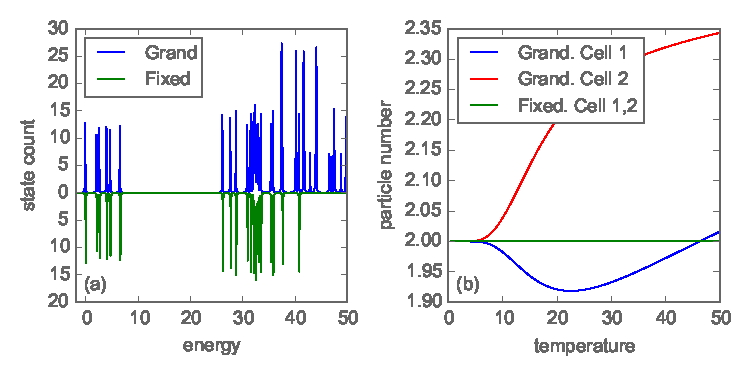
\includegraphics{fixed_charge_approximation}
  \caption{
  (a) Low-energy density of states of the exact grand canonical and the
  approximative fixed charge two-cell QCA system. For small energies the curves
  agree perfectly (up to $E \lesssim 35$). (b) Particle number per cell over
  temperature for the same two-cell system. The curves diverge for $T \gtrsim
  10$.
  }
  \label{fig:fixed_charge_approximation}
\end{figure}
%
%
\begin{figure}
  \center
  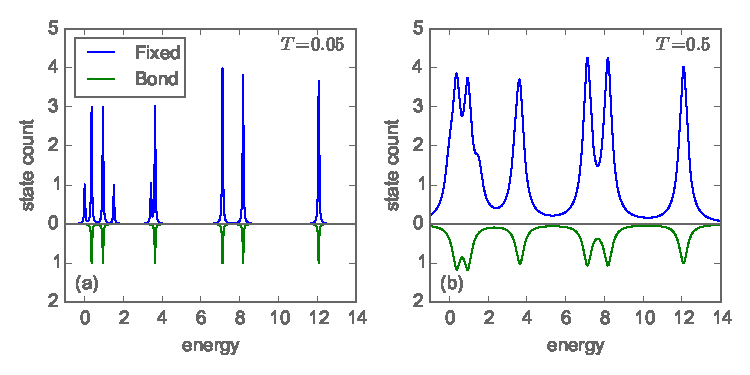
\includegraphics{bond_approximation1}
  \caption{
  (a) Low-energy density of states of a one-cell QCA system for both the fixed
  charge and the bond model. The bond approximation only reproduces the triplet
  states, but omits the singlet states. The ``measurement'' temperature is
  indicated. (b) The same spectrum, but ``measured'' at a higher temperature. At
  large enough temperatures the singlet-triplet splitting is ``washed out'': The
  singlet and triplet peaks are no longer separately resolved and the bond
  model's state corresponds to four fixed charge states at roughly the same
  energy.
  }
  \label{fig:bond_approximation1}
  % parameters: V_1 = 20, boa = 2, U = 1E6, q = 0, P_D = 1, T = 1, mu = 0
\end{figure}
%
The fixed charge approximation is a Hilbert space truncation where we only keep
the states with exactly two electrons per cell.
Fig.~\ref{fig:fixed_charge_approximation}(a) compares the density of states of
the fixed charge model against the exact grand canonical system. It reproduces
the low-energy spectrum, in the plot up to $E \lesssim 35$, exactly. Therefore,
as long as the two-electrons-per-cell sector is lowest in energy and the
temperature is low compared to the energy gap to the next charge sector, the
model works perfectly. Fig.~\ref{fig:fixed_charge_approximation}(b) plots the
number of particles per cell over temperature and demonstrates the breakdown of
the approximation, precisely as the temperature does become comparable to this
energy gap. Whereas the fixed charge model gives, per definition, a constant
number of particles over the whole temperature range, the grand canonical
system's cell occupancy starts diverging from two electron per cell at around $T
\sim 10$. This roughly corresponds to the energy states the fixed charge model
missed at $E \sim 40$. A small deviation from exactly two electrons per cell is
not detrimental to QCA, a cell occupied by only one or by three electrons,
however, renders QCA non-functional. As we already said in the beginning of this
chapter, we often use the fixed charge model as the starting point and assume,
without further investigation, that a practical QCA implementation can be tuned
to be in the right charge regime at a given temperature.

As a side note, we calculate the density of states graphs by folding the energy
eigenvalues of the system---a delta function energy spectrum---with a Lorentzian
with the half-width at half-maximum set by a ``measurement'' temperature. Very
roughly speaking, this corresponds to a photoemission / inverse photoemission
spectroscopy experiment at this temperature.

The bond model neglects doubly occupied states and represents the four states of
a bond---one singlet and three triplets---with only one single bond state. The
model thus assumes that singlet and triplet states are energetically degenerate,
but we had already asserted that we might expect a small singlet-triplet
splitting. Fig.~\ref{fig:bond_approximation1}(a) shows the density of states of
a single QCA cell for both the fixed charge and the bond model. The
nearest-neighbour Coulomb energy is $V_1 = 20$, the hopping is $t=1$. A driver
cell placed at a distance $d/a = 3$ to the left of the single cell sets an
input. We have chosen the driver cell's polarization to be $P_D = 1$. Indeed, each
bond state corresponds to three fixed charge states---the triplet---and one
``close-by'' state---the singlet. They are not energetically equivalent, but
split by a small energy gap, $\Delta E_S$, the singlet-triplet splitting. The
bond model picks out the triplet states and in fact exactly reproduces those
states. Just as the fixed charge model the bond model truncates the Hilbert
space, but the retained states are exact. Evidently, the bond model keeps one of
the three triplet states, but discards the other two triplet and the singlet
states. We speculate that, similar to the antiferromagnetic Heisenberg coupling
constant $J$ emerging in the low energy limit of the Hubbard model (with $J \sim
\frac{t^2}{U}$) \cite{Auerbach}, here, for the ground state virtual excitations
to high energy doubly occupied states lower the energy of the singlet state
compared to the triplet state. As the bond model misses those doubly occupied
states it cannot accommodate singlet states and hence reproduces the triplet
states. Consequently, we cannot hope that the bond model correctly reproduces
ground state or low-energy properties. However, we assert that as long as the
singlet-triplet splitting is ``washed out'', that is, as long as the temperature
is much larger than the singlet-triplet gap, $T \gg \Delta E_S$, the
approximation should give correct results. At high enough temperatures the
system no longer ``sees'' the difference between the singlet and the triplet
states. This is illustrated in Fig.~\ref{fig:bond_approximations1}(b) where the
spectrum is ``measured'' at a higher temperature. The singlet and triplets are
no longer resolved separately.  Instead, each bond state corresponds to four
fixed charge states at roughly the same energy. The figure shows all six bond
states of the single cell, the complete spectrum apart from the doubly occupied
states. As this cell is perturbed by a nearby driver cell with $P_D = 1$, the
ground state is qualitatively closest to the logic 1 state, or $\ket{2}$ in
Fig.~\ref{fig:bond}.  Similarly, the first excited state is similar to
$\ket{1}$, or logic 0, and the four higher energy states correspond to
$\ket{4}$, $\ket{5}$, $\ket{3}$, and $\ket{6}$, in that order. Of course, in
general the energy eigenstates are a mixture of all basis states, but we can
still characterize them by their most dominantly contributing basis state. As
this a non-charge-neutral system $q=0$ with a relatively small cell-cell
distance $d/a = 3$, charge buildup tends to push the electrons to the far edge
of the cell, thus making $\ket{4}$ lower in energy than $\ket{6}$.

Since the bond model ignores the singlet-triplet splitting it is important to
understand how the gap $\Delta E_S$ depends on various system parameters. To
that end we picked out a few selected singlet-triplet states from the spectrum
in Fig.~\ref{fig:bond_approximation1}(a) as examples. Contrary to expectations,
for those states the gap $\Delta E_S$ did not change significantly with the
on-site Coulomb repulsion $U$, however, it did decrease with decreasing $d$, the
cell-cell distance. Most importantly, for the nearest-neighbour Coulomb energy
$V_1$ we found $\Delta E \sim \frac{1}{V_1^p}$. The exponent is $p \sim 3$ when
the cell ``sees'' a biasing external potential (e.g.\ $P_D = \pm 1$) and $p \sim
1$ otherwise (e.g.\ $P_D = 0$). Even though our method is anything but rigorous
and the obtained results very likely not universally true, the findings should
nonetheless give a good enough idea of the principle trends. Quite generally,
the higher the overall Coulomb potential (large $V_1$, small $d$), the smaller
the singlet-triplet splitting and, conceivably, the more accurate the bond
approximation. Consequently, we expect the approximation to work as long as the
singlet-triplet splitting is ``washed out,'' that is, as long as the temperature
is much bigger than the gap $\Delta E$. As a very, very rough estimate we come
up with $T \gg \frac{t^2}{V_1}$. Of course, we also need $T \ll U$ so that the
doubly occupied states are gapped out. Outside of this loosely defined regime,
the bond model can and does go terribly wrong.

To illustrate the limitations of the bond approximations we now look at a two
cell system: a straight horizontal line of two cells with a driver cell to the
left. Fig.~\ref{fig:bond_approximation2} shows the spectra and output
polarizations of a two-cell wire for two different Coulomb energies, $V_1 = 20$
and $V_1 = 100$. Otherwise the parameters are the same as for the one-cell
system in the previous graph. In particular, the spectrum in
Fig.~\ref{fig:bond_approximation2}(a) is exactly the same as in
Fig.\ref{fig:bond_approximation1}(a) except that we have added one more cell to
the system. Each bond state now corresponds to 16 ($4 \cdot 4$) fixed charge
states. Looking at the four lowest-energy peaks in the spectrum, we see that the
bond model exactly reproduces the 9 triplet-triplet states, but misses the three
singlet-triplet and the three triplet-singlet states (in the graph the
corresponding two peaks are hardly distinguishable), as well as the single
singlet-singlet ground state. The four lowest bond states should roughly
correspond to both cells being aligned with the driver cell (the ground state),
only one of the two cells being aligned with the driver cell, and both cells
being anti-aligned with the driver cell. Higher energy states have at least one
of the cells not in the preferred diagonal states $\ket{1}$ and $\ket{2}$, with
electrons occupying predominantly the edge of a cell. Arguably, 
the spectra of the fixed charge and the bond model in
Fig.~\ref{fig:bond_approximation2}(a) do not look very similar. Consequently,
the polarization curves in Fig.~\ref{fig:bond_approximation2}(b) do not agree,
especially at low temperatures. In fact, it is rather remarkable that given the
widely dissimilar spectra the polarizations actually do agree relatively well at higher
temperatures, $T > 1$. The bond model only reproduces the most populous energy
states of the exact spectrum. Apparently, that is enough to give (almost)
correct results at high temperatures. The lower the temperature, the more
important become the few lowest lying energy states which the bond model misses.
Very roughly speaking, the temperature where the bond model's polarization
becomes accurate also matches the temperature where we saw the singlet-triplet
splitting being washed out in Fig.~\ref{fig:bond_approximation1}(b), they are at
least of the same order of magnitude. For the much larger Coulomb energy $V_1 =
100$ the spectra look much more alike, qualitatively, even though the bond model
obviously still does not resolve all the lines of the exact density of states,
and consequently the approximation works much better,
Fig.~\ref{bond_approximation2}(a) and (b). The polarization curves agree down to
much lower temperatures and even the discrepancy for the ground state
polarizations is much reduced. Compared to the $V_1 = 20$ system the ground
state polarization is much larger and, generally, the higher the cell
polarization, the better the agreement between bond and fixed charge model. We
also note that in the spectrum the peaks are much more spaced out, compared to
the $V_1 = 20$ system. Thus the system retains larger cell polarizations up to
much higher temperatures.

The polarization of the fixed charge model shows a curious bump at low
temperatures, for example in Fig.~\ref{fig:bond_approximation2}(b) and
similarly, if less visibly, in Fig.~\ref{fig:bond_approximation2}(d).
Apparently, the ground state is not the most polarized state. Maximum
polarization is reached at a small, but finite temperature. At the same time,
for the bond model the ground state is the most polarized state and generally
its $T=0$ polarization is larger than that of the fixed charge model.
Interestingly, the bond model's ground state polarization is largely independent
of the magnitude of the driver polarization and also only weakly influenced by
the cell-cell distance $d$, especially for charge-neutral cells where no charge
buildup occurs. Instead, it is predominantly set by $V_1$, and thus by $V_1/t$
and the energy gap $\Delta V = V_1 - V_0$. Without an external perturbation such
as a non-zero driver polarization the ground state polarization is zero, of
course. But any infinitesimal external perturbation will instantly see the bond
model's ground state polarization snap to its full value. We interpret this
behaviour as the ground state actually consisting of two energetically
degenerate states, corresponding to $\pm P_{gs}$, where $P_{gs}$ is the full
ground state polarization for a given $V_1$. The smallest perturbation lifts
this degeneracy and sees the system snapping to either $+P_{gs}$ or $-P_{gs}$.
Now the bond model's ground state corresponds to the fixed charge model's
triplet state---one of the lower lying excited states, but not the ground state.
The true ground state of the more exact model is a single singlet state, a
superposition of the $+P_{gs}$ and $-P_{gs}$ (and other) states. Therefore the
polarization of the true ground state is generally smaller in magnitude than the
polarization of the corresponding two triplet states, explaining the low
temperature bump in the polarization curve and the larger polarization of the
bond model's ground state.
%
\begin{figure}
  \center
  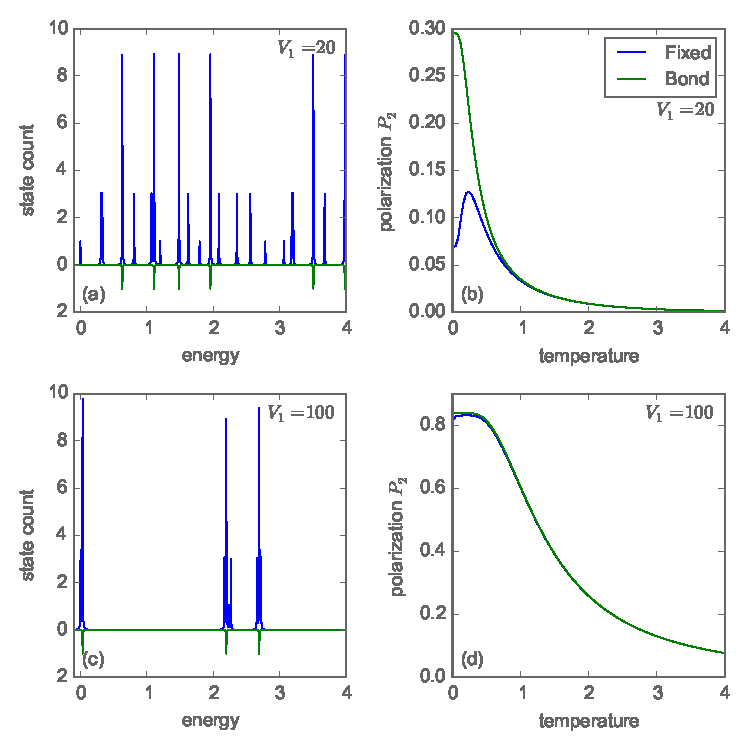
\includegraphics{bond_approximation2}
  \caption{
  The two-cell fixed charge and bond systems at $V_1 = 20$ and $V_1 = 100$.
  (a)(c) Low-energy density of states. (b)(d) Output polarization $P_2$ over
  temperature. For a small Coulomb repulsion the density of states curves look
  qualitatively very different (a) and the bond approximation does not work very
  well (b). At a larger Coulomb repulsion the density of states curves look much
  more alike (c) and the bond approximation works much better (d).
  }
  \label{fig:bond_approximation2}
\end{figure}
%
% TODO: mention which value of U we are using for the simulations; (it should be
% U=1E6 for all plots so far)


The Ising approximation is derived as an effective low-energy model from the
bond Hamiltonian. It is therefore qualitatively different from the previous two
approximations: It is not merely a Hilbert space truncation. \emph{A priori}
its states need not exactly correspond, neither energetically nor qualitatively, to either the bond or the fixed charge
model. Of course, in the limit where the assumptions in the derivation become
exact, the Ising model's states should resemble the bond model's states
accurately. Specifically, the derivation assumed $E \approx V_0$ ($E$ the energy
of the whole system) and therefore $t \ll \Delta V$, as well as $\Delta V \gg
T$. The neglected edge states need to be gapped out. Additionally, cells are
assumed to be isolated, so the Ising model presumably requires reasonably large
cell-cell distances. The Ising model also inherits the limits of the bond model and we
would expect $T \gg \Delta E_S$ and $T \ll U$ as requirements for the Ising
model as well. It is important to keep in mind that the Ising model is not a low-energy
model for the more exact fixed charge Hamiltonian---it is derived as the
low-energy limit of the bond model, which, however, is not an accurate
low-energy description of the fixed charge system. The Ising model with its only
two states per cell can never accurately capture the lowest lying states of the
fixed charge model, which are, for a multi-cell system, a mixture of
singlet-triplet states across cells. The approximation can also not hope to
capture non-charge neutral systems and more specifically charge buildup
correctly. It simply lacks the edge states that would be the manifestation of
charge buildup, as discussed in the example of the one-cell bond system above.
We had seen in the derivation of the Ising model that the lack of
charge-neutrality is very problematic for the QCA approach in general.
Consequently, we will concentrate on charge neutral systems, $q = \frac{1}{2}$,
for the remainder of the chapter. For the following calculations we do not use
the derived $J_{kl}$ and $J^{\prime}_{kl}$ terms, but some all Coulomb
interactions exactly.

To understand how the Ising approximation works we again start by looking at the
density of states for a one-cell system, Fig.~\ref{fig:ising_approximation1}(a).
We have plotted both the fixed charge and the bond model for comparison and now
use slightly different system parameters. The nearest-neighbour Coulomb energy
is $V_1 = 100$, the cell-cell distance is $d/a = 4$, the driver cell is only
slightly polarized with $P_D = 0.1$, and, as always, the hopping is $t=1$. We are in for a surprise! Evidently, the
Ising model reproduces the singlet states and not the bond model's triplet
states. In line with this observation, the Ising model exactly matches the fixed
charge model's ground state polarization, but misses the triplet-bump at $T \sim
0.05$, Fig.~\ref{fig:ising_approximation1}(b). Thus, for the one-cell system the
Ising approximation unexpectedly captures the system's ground state correctly.
Apparently, even though we had derived the Ising model from the bond
Hamiltonian, it does not really resemble the bond model. Instead its states are
of singlet character. It even gets the ground state right, after we had just
asserted that it cannot possibly be a low-energy description of the fixed charge model.
In short, the Ising model's behaviour is very confusing. To lift the confusion,
we first note, that even though the Ising model correctly captures the ground
state of the single cell system, this is not true in general, for larger
systems, as we will see in a moment. It also is not a low-energy effective model, because
even for the one-cell system it only reproduces the ground state, but not the
first and second excited states. Second, we need to be very careful when we talk
about the bond model. The bond Hamiltonian is simply a spinless model that does
not distinguish between singlet and triplet states. In contrast, the bond model
uses a concrete basis and we saw that it chooses the triplet states. Therefore,
the bond Hamiltonian, from which we derived the Ising model, and the bond model
are not equivalent. With its choice of basis the Ising model captures the
singlet states. This makes sense in so far as the Ising model is derived as the
low-energy effective model and the singlet states are the lowest energy states.
The Ising and bond model states are therefore different energetically and
qualitatively. Still, in the limit where the Ising model becomes exact, the
singlet-triplet splitting should go to zero and the states of the two models
will become equivalent. On second thought, the fact that the Ising model exactly
reproduces the ground state of the one-cell system is maybe not as surprising:
We had derived the Ising model precisely for a single cell and as it captures
the singlet states, that is what we get. Apparently, the perturbation of the
external driver cell does not change that fact. Close inspection of the energy
gap between the Ising model's only two states, however, as compared to the
equivalent energy gap between the fixed charge model's two lowest energy singlet
states, show that the fixed charge and Ising states are not exactly the same,
energetically. The difference is hardly discernible in the plotted spectrum, but
more pronounced for different system parameters. This is not surprising, given
that the Ising approximation is a effective model and used several assumptions
in its derivation. Indeed, for the single-cell system we can study the energy
gap for the Ising as compared to the fixed charge model and find that they are
in better agreement for larger $V_1$, smaller $t$, and larger cell-cell distance
$d/a$ (although the difference becomes constant for large enough $d/a$,
presumably when the cells are spaced far enough apart to not influence each
other's hopping), exactly confirming the assumptions and limits of our
derivation.
% mention: bond fully polarized here, for q = 1/2
% would not hurt to explicitly mention that energy gap error becomes large for
% very small d/a, specifically d/a < 2 --- here, Ising very explicitly breaks
% down
% maybe explain here: Ising weirdness is not a shortcoming of our derivation,
% but a consequence of pressing QCA in a two-state basis


% two sets of conditions for Ising model

% 
% spectra look qualitatively more alike for larger P_D---we only use P_D=0.1
% spectra look more alike for smaller d/a and for larger V1

% also need to mention that models tend to agree for fully polarized cells ---
% hence I need to look at a regime where the system is not fully polarized

%
\begin{figure}
  \center
  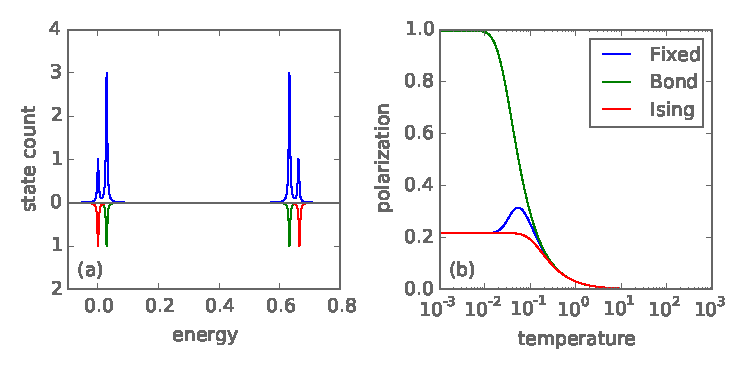
\includegraphics{ising_approximation1}
  \caption{\ldots}
  \label{fig:ising_approximation1}
  % parameters: V1 = 100, boa = 3, P_D = 0.1, q = 0.5
\end{figure}
%
%
\begin{figure}
  \center
  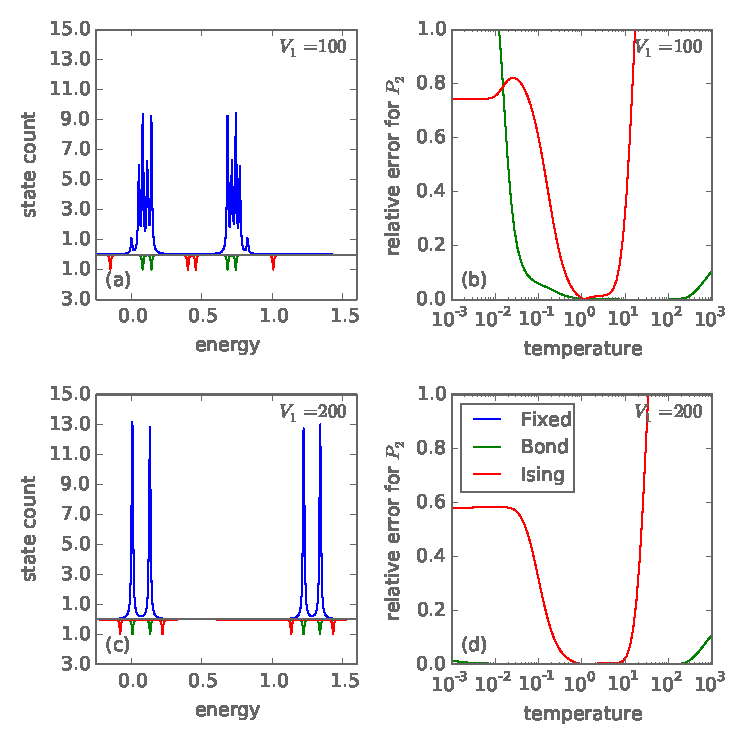
\includegraphics{ising_approximation2}
  \caption{\ldots}
  \label{fig:ising_approximation2}
  % parameters: V1 = 100, 200, boa = 3, P_D = 0.1, q = 0.5, U=1E3
\end{figure}
%
%
\begin{figure}
  \center
  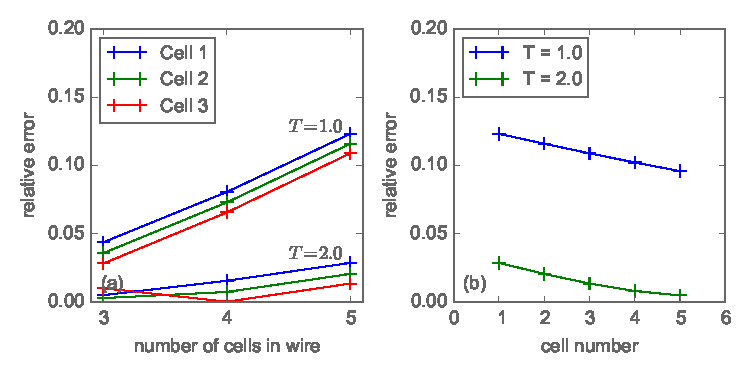
\includegraphics{ising_approximation3}
  \caption{\ldots}
  \label{fig:ising_approximation3}
  % parameters: V1 = 100, boa = 3, P_D = 0.1, q = 0.5
\end{figure}
%


% TODO: mention which plots are q=0 and which ones are q=1/2
% TODO: Include partition function argument / explanation somewhere?
% TODO: good argument why there are two degenerate ground states for the bond
% model? (triplet, symmetry argument?)
% TODO: Is there a better explanation why bond chooses triplet and Ising singlet
% states?
